\documentclass{scrartcl}
\usepackage{tikz}
\usetikzlibrary{arrows,automata}
\usepackage{comment}
\usepackage[linguistics]{forest}
\usepackage{textcomp}
\usepackage{makecell}
\usetikzlibrary{automata,positioning}
\usepackage{amsmath,amsfonts,amssymb}

\begin{document}
\hfuzz=\maxdimen
\tolerance=10000
\hbadness=10000
\begin{center}
Wen Liang(\texttt{Wen\_Liang@student.uml.edu}) 01724877
\end{center}
\section*{2.1}
\subsection*{a.}
derivation:\qquad$
E\Rightarrow T\Rightarrow F\Rightarrow a$
\\
\\
\begin{forest}
[E
[T
[F
[a]
]
]
]
\end{forest}

\subsection*{b.}
derivation:\qquad $ E\Rightarrow E + T\Rightarrow T + T\Rightarrow F + T \Rightarrow a + T\Rightarrow a+F\Rightarrow a+a $
\\
\\
\begin{forest}
	 for tree={
		if n children=0{
			tier=terminal,
		}{},
	}
	[E
     [E
     [T
     [F
     [a]
     ]
     ]
     ]
     [+]
	 [T
	 [F[a]
	 ]
	 ]
	 ]
\end{forest}

\subsection*{c.}
derivation:\qquad $ E\Rightarrow E + T\Rightarrow E + T + T\Rightarrow T+ T + T \Rightarrow F + T + T\Rightarrow a+T+T\Rightarrow a+F+T\Rightarrow a+a+T \Rightarrow a+a+F \Rightarrow a+a+a $
\\
\\
\begin{forest}
	for tree={
		if n children=0{
			tier=terminal,
		}{},
	}
	[E
	[E[E[T[F[a]]]][+][T[F[a]]]]
	[+]
	[T[F[a]]]
	]
\end{forest}
\\
\\
\subsection*{d.}
derivation:\qquad $ E\Rightarrow T\Rightarrow F\Rightarrow (E) \Rightarrow (T) \Rightarrow (F)\Rightarrow ((E))\Rightarrow ((T)) \Rightarrow ((F)) \Rightarrow ((a)) $
\\
\\
\begin{forest}
	for tree={
		if n children=0{
			tier=terminal,
		}{},
	}
	[E[T[F
	[(] [E[T[F [(] [E[T[F[a] ] ]]  [)]   ]]]
	[)]
	]]
	]
\end{forest}


\section*{2.4}
\subsection*{b.}
$S\rightarrow 0R0 \mid 1R1 \mid \epsilon
\\
R\rightarrow 0R  \mid 1R \mid\epsilon$



\subsection*{c.}
$S\rightarrow 0\mid 1\mid 00S\mid 01S\mid 10S\mid 11S
$
\subsection*{e.}
$S\rightarrow 0S0\mid 1S1\mid 0\mid 1\mid \epsilon
$

\subsection*{f.}
$S\rightarrow S$


\section*{2.5}
\subsection*{a.}
This is a regular language, so the language has a DFA. We can easily
convert the DFA into a PDA by using the same states and transitions and never
push nor pop anything from the stack. If A contain at least three 1s, then accept; otherwise, reject.
\\
\\
\\
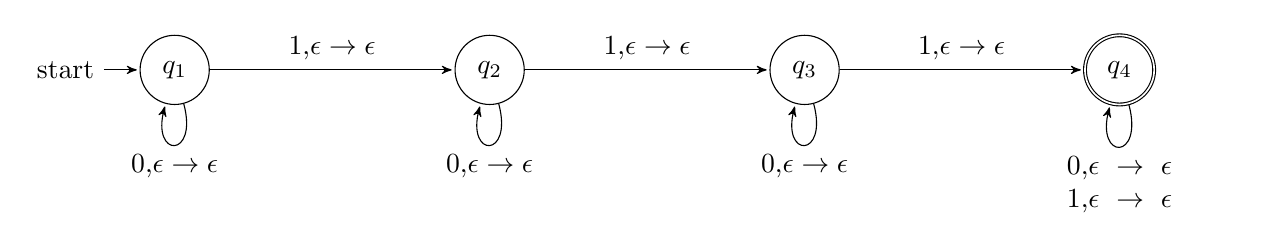
\begin{tikzpicture}[>=stealth',shorten >=1pt,auto,node distance=4cm]


\node[initial,state	]   (q1)      				{$q_1$};
\node[state] 	  (q2) [right of=q1]  	{$q_2$};
\node[state] 	  (q3) [right of=q2]  	{$q_3$};
\node[state,accepting] 	  (q4) [right of=q3]  	{$q_4$};

\path[->] (q1)  edge[loop below]	  	node{0,$\epsilon \rightarrow \epsilon$}	(q1)
edge	  node{1,$\epsilon \rightarrow \epsilon$}	(q2)

(q2)  edge[loop below]	 node{0,$\epsilon \rightarrow \epsilon$} 		(q2)
edge  	node{1,$\epsilon \rightarrow \epsilon$}  	(q3)

(q3)  edge[loop below]	 node{0,$\epsilon \rightarrow \epsilon$} 		(q3)
edge  	node{1,$\epsilon \rightarrow \epsilon$}  	(q4)
(q4)  edge[loop below]	 node[text width=3cm,align=center]{0,$\epsilon \rightarrow \epsilon$\\1,$\epsilon \rightarrow \epsilon$} 		(q4);

\end{tikzpicture}

\subsection*{b.}
We will nondeterministically guess if the string has only one symbol in which case we accept it without using the stack;  otherwise, we push the first
symbol read onto the stack. Then we will read every other symbol and nondeterministically guess if that is the last symbol read. If the last symbol read then matches the symbol on the stack and there is no more input we accept. Otherwise we reject.
\\
\\
\\
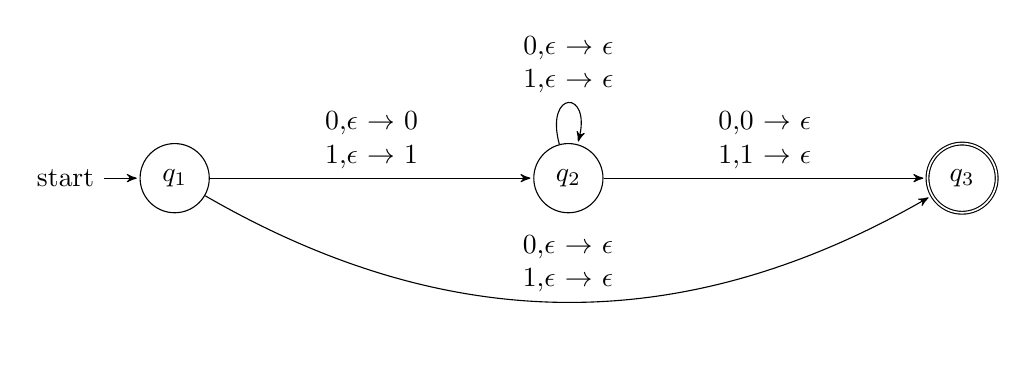
\begin{tikzpicture}[>=stealth',shorten >=1pt,auto,node distance=5cm]


\node[initial,state	]   (q1)      				{$q_1$};
\node[state] 	  (q2) [right of=q1]  	{$q_2$};
\node[state,accepting] 	  (q3) [right of=q2]  	{$q_3$};

%[text width=1cm,align=center] {0,1,2\\3,4,5} (q_0);


\path[->] (q1)  edge	  	node[text width=3cm,align=center]{0,$\epsilon$ $\rightarrow$ 0 \\ 1,$\epsilon$ $\rightarrow$ 1} 	(q2)
	edge[bend right]	  	node[text width=3cm,align=center]{0,$\epsilon$ $\rightarrow$ $\epsilon$\\1,$\epsilon$ $\rightarrow$ $\epsilon$} 	(q3)

(q2)  edge[loop above]	  	node[text width=3cm,align=center]{0,$\epsilon$ $\rightarrow$ $\epsilon$\\1,$\epsilon$ $\rightarrow$ $\epsilon$}  	(q2)
  edge  	node[text width=3cm,align=center]{0,0 $\rightarrow$ $\epsilon$\\1,1 $\rightarrow$ $\epsilon$} 	(q3);

\end{tikzpicture}

\subsection*{c.}
The stack is not needed here at all. Therefore we will read the
input and only accept if the length is odd, that is after the first symbol read or every other symbol read thereafter if it is the final symbol read.
\\
\\
\\
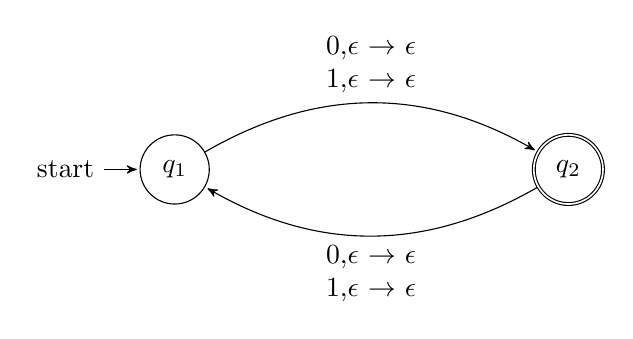
\begin{tikzpicture}[>=stealth',shorten >=1pt,auto,node distance=5cm]


\node[initial,state	]   (q1)      				{$q_1$};
\node[state,accepting] 	  (q2) [right of=q1]  	{$q_2$};


%[text width=1cm,align=center] {0,1,2\\3,4,5} (q_0);


\path[->] (q1)  edge[bend left]	  	node[text width=3cm,align=center]{0,$\epsilon$ $\rightarrow$ $\epsilon$ \\ 1,$\epsilon$ $\rightarrow$ $\epsilon$} 	(q2)

(q2)  edge[bend left]	  	node[text width=3cm,align=center]{0,$\epsilon$ $\rightarrow$ $\epsilon$\\1,$\epsilon$ $\rightarrow$ $\epsilon$}  	(q1);


\end{tikzpicture}

\subsection*{d.}
The PDA detect the input string and pushes the symbols onto the stack. At some point it nondeterministically guesses where the middle is. It checks to see if the middle symbol is a 0. Then it scans the rest of the string, and pops one character off the stack for each character scanned. If when it finishes scanning the input , and of course correctly guessed the middle, and the stack is empty, then accept. Otherwise, reject.\\
\\
\\
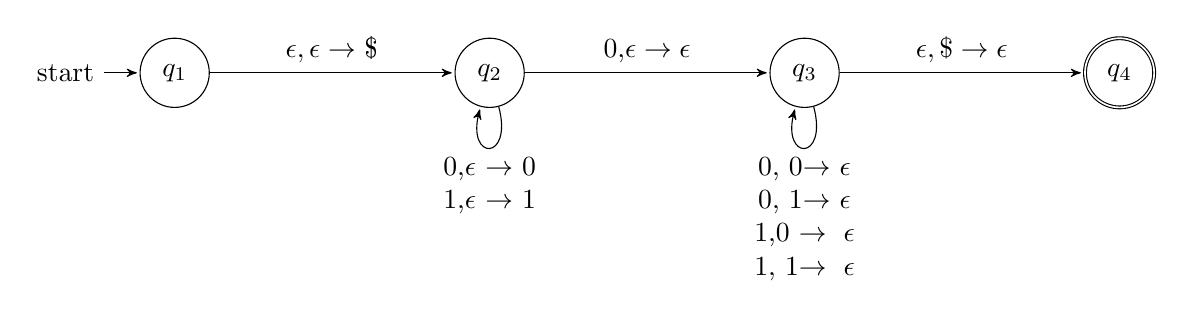
\begin{tikzpicture}[>=stealth',shorten >=1pt,auto,node distance=4cm]


\node[initial,state	]   (q1)      				{$q_1$};
\node[state] 	  (q2) [right of=q1]  	{$q_2$};
\node[state	]   (q3)[right of=q2]      				{$q_3$};
\node[state,accepting] 	  (q4) [right of=q3]  	{$q_4$};

%[text width=1cm,align=center] {0,1,2\\3,4,5} (q_0);


\path[->] (q1)  edge	  	node{$\epsilon,\epsilon \rightarrow$ \$}	(q2)

(q2)  edge[loop below]	  	node[text width=3cm,align=center]{0,$\epsilon$ $\rightarrow$ 0\\1,$\epsilon$ $\rightarrow$ 1}  	(q2)

 (q2)  edge	  	node{0,$\epsilon \rightarrow \epsilon$}	(q3)
 (q3)  edge[loop below]	  	node[text width=3cm,align=center]{0, 0$\rightarrow$ $\epsilon$\\0, 1$\rightarrow$ $\epsilon$\\1,0 $\rightarrow \epsilon$\\1, 1$\rightarrow \epsilon$}  	(q3)
 (q3)  edge	  	node{$\epsilon,\$ \rightarrow \epsilon$}	(q4);
 

\end{tikzpicture}

\subsection*{e.}
Informal Description: We begin by pushing the symbols read onto the stack. At each
point we will nondeterministically guess if the middle of the string has been reached or if the next symbol read is the middle of the string and will not be put on the stack. Then we pop off the symbols from the stack if they match the input symbols read. If the symbols popped are exactly the same symbols that were pushed on earlier and the stack empties as the input is finished, then accept. Otherwise, reject.
\\
\\
\\
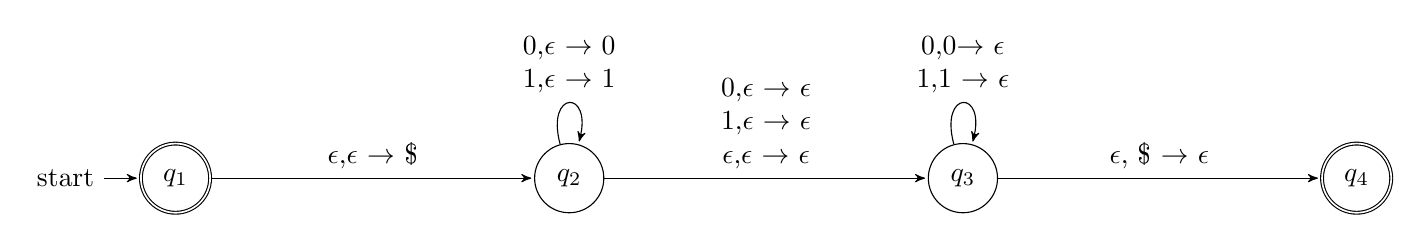
\begin{tikzpicture}[>=stealth',shorten >=1pt,auto,node distance=5cm]


\node[initial,state,accepting	]   (q1)      				{$q_1$};
\node[state] 	  (q2) [right of=q1]  	{$q_2$};
\node[state] 	  (q3) [right of=q2]  	{$q_3$};
\node[state,accepting] 	  (q4) [right of=q3]  	{$q_4$};

%[text width=1cm,align=center] {0,1,2\\3,4,5} (q_0);


\path[->] (q1)  edge	  	node[text width=3cm,align=center]{$\epsilon$,$\epsilon$ $\rightarrow$ \$} 	(q2)

(q2)  edge[loop above]	  	node[text width=3cm,align=center]{0,$\epsilon$ $\rightarrow$ 0\\1,$\epsilon$ $\rightarrow$ 1}  	(q2)
  edge	  	node[text width=3cm,align=center]{0,$\epsilon$ $\rightarrow$ $\epsilon$\\1,$\epsilon$ $\rightarrow$ $\epsilon$ \\ $\epsilon$,$\epsilon$ $\rightarrow$ $\epsilon$}  	(q3)
(q3)  edge[loop above]	  	node[text width=3cm,align=center]{0,0$\rightarrow$ $\epsilon$\\1,1 $\rightarrow$ $\epsilon$}  	(q3)
  edge	  	node[text width=3cm,align=center]{$\epsilon$, \$ $\rightarrow$ $\epsilon$}  	(q4);
\end{tikzpicture}

\subsection*{f.}
Note: Since, no derivations terminate, the CFG cannot accept any strings, including the empty. The PDA consists of one state that does not accept.
\\
\\
\\
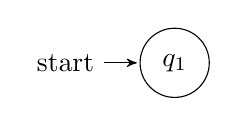
\begin{tikzpicture}[>=stealth',shorten >=1pt,auto,node distance=5cm]


\node[initial,state	]   (q1)      				{$q_1$};


\end{tikzpicture}




\section*{2.6}
\subsection*{a.}
$S\rightarrow TaT\\
T\rightarrow TT\mid aTb\mid bTa\mid a\mid \epsilon$
\subsection*{b.}
$S\rightarrow T\mid aU \mid Vb\\
T\rightarrow aT\mid Ta \mid bT \mid Tb\mid ba\\
U\rightarrow aU \mid W\\
V\rightarrow Vb \mid W\\
W\rightarrow aWb\mid \epsilon
$

\subsection*{c.}
$ S\rightarrow TX\\
T\rightarrow 0T0\mid 1T1 \mid \# X\\
X\rightarrow 0X \mid 1X \mid \epsilon $

\subsection*{d.}
$ S\rightarrow A\# B \# A \mid B \# A \mid A \# B \mid B\\
B\rightarrow aBa \mid bBb \mid \# \mid \# A \# \\
A\rightarrow aA \mid bA \mid \#A \mid \epsilon$


\section*{2.9}
$S\rightarrow R_{ab}C \mid AR_{bc}\\
R_{ab}\rightarrow aR_{ab}b \mid \epsilon\\
R_{bc}\rightarrow bR_{bc}c \mid \epsilon\\
C\rightarrow Cc \mid \epsilon\\
A\rightarrow Aa \mid \epsilon$\\ \\
This grammar is ambiguous. Because the string $\epsilon$ can be derived by choosing $R_{ab}$C,but both$ R_{ab}$ and C can generate $\epsilon$; and $\epsilon$ can be derived by choosing $AR_{bc}$, but both $R_{bc}$ and A can yield $\epsilon$.

\section*{2.10}
1. Nondeterministically branch to either step 2 or step 6.\\
2. Read and push a.\\
3. Read b, while popping a.\\
4. if b finish when stack is empty,skip c on input and accept\\
5. Skip a on the input\\
6. Read and push b\\
7. Read c, while popping b.\\
8. if c finish when stack is empty,accept

\section*{2.11}
1. Place the marker symbol \$ and the start variable E on the stack.\\
2. Repeat the following steps forever. \\
3. if the top of stack is the variable E, pop it and nondeterministically push either E+T or T into the stack.\\
4. if the top of stack is the variable T, pop it and nondeterministically push either T  $\times$  F or F into the stack.\\
5. if the top of the stack is the variable F, pop it and nondeterministically push either (E) or a into the stack.\\
6. if the top of the stack is a terminal symbol, read the next symbol from the input and compare it to the terminal in the stack. If they match, repeat. If they do not match, reject on this branch of the nondeterminism.\\
7. if the top of the stack is the symbol \$, enter the accept state. Doing so accepts the input if it has all been read.\\
\\
The formal definition of the equivalent PDA is (Q,$\Sigma$,$\Gamma$,$\delta$,$q_1$,F),where Here Q = \{$q_1$,$q_2$\}; $\Sigma$ = \{+,$\times$,(,),a\}; and $\Gamma$ =\{E, T, F\} $\cup$ $\Sigma$; F =\{$q_2$\}. The transition function $\delta$ : Q $\times$ ${\Sigma}_\epsilon$  $\times$ $\Gamma_\epsilon$ $\rightarrow$ P(Q $\times$ $\Gamma_\epsilon$ ) is given as follows.\\
\\
\begin{equation}
{\delta}(q,x,y)=\left\{
\begin{array}{rcl}
\{(q_2,\epsilon)\} & & { if q=q_1,x=\epsilon, y=\$}\\
\{(q_1,E+T),(q_1,T)\} & & {if q=q_1,x=\epsilon,y=E}\\
{(q_1,T \times F), (q_1, F)} & & {if q=q_1, x=\epsilon,y=T}\\
{(q_1,(E)),(q_1,a)} & & {if q=q_1,x=\epsilon,y=F}\\
{(q_1,\epsilon)} & & {if q=q_1,x=y}\\
\end{array} \right.
\end{equation}

\section*{2.12}
1. Place the marker symbol \$ and the start variable E on the stack.\\
2. Repeat the following steps forever. \\
3. if the top of stack is the variable R, pop it and nondeterministically push either XRX or S into the stack.\\
4. if the top of stack is the variable S, pop it and nondeterministically push either aTb or bTa into the stack.\\ 
5. if the top of the stack is the variable T, pop it and nondeterministically push either XTX, X or $\epsilon$ into the stack.\\
6. if the top of the stack is the variable X, pop it and nondeterministically push either a or b into the stack.\\
7. if the top of the stack is a terminal symbol, read the next symbol from the input and compare it to the terminal in the stack. If they match, repeat. If they do not match, reject on this branch of the nondeterminism.\\
8. if the top of the stack is the symbol \$, enter the accept state. Doing so accepts the input if it has all been read.\\
\\

The formal definition of the equivalent PDA is (Q,$\Sigma$,$\Gamma$,$\delta$,$q_1$,F),where Here Q = \{$q_1$,$q_2$\}; $\Sigma$ = \{a,b\}; and $\Gamma$ =\{R, S, T, X\} $\cup$ $\Sigma$; F =\{$q_2$\}. The transition function $\delta$ : Q $\times$ ${\Sigma}_\epsilon$  $\times$ $\Gamma_\epsilon$ $\rightarrow$ P(Q $\times$ $\Gamma_\epsilon$ ) is given as follows.\\
\\
\begin{equation}
{\delta}(q,x,y)=\left\{
\begin{array}{rcl}
\{(q_2,\epsilon)\} & & { if q=q_1,x=\epsilon, y=\$}\\
\{(q_1, XRX),(q_1, S)\} & & {if q=q_1,x=\epsilon,y=R}\\
{(q_1, aTb), (q_1, bTa)} & 	& {if q=q_1, x=\epsilon,y=S}\\
{(q_1, XTX),(q_1, X), (q_1, \epsilon)} & & {if q=q_1,x=\epsilon,y=T}\\
{(q_1, a),(q_1, b)} & & {if q=q_1,x=\epsilon, y=X}\\
{(q_1, \epsilon)} & & {if q=q_1,x=y}\\
\end{array} \right.
\end{equation}

\section*{2.13}
\subsection*{a.}
L(G) is the set of strings of 0s and \#s that either contain exactly 2 \#s and any number of 0s, or contain exactly 1 \# and the number of 0s to the right of the \# is twice the number of 0s to the left.

 
\subsection*{b.}
Assume L(G) is regular. Let A=L(G) $\cap$ $0^*$\#$0^*$. If L(G) is regular, so is A. Let p be the pumping length for A given by the pumping lemma for regular languages. Consider the string w = $0^p$\#$0^{2p}$. Because $\mid$ w $\mid$ $>$ p and w $\in$ A, the pumping lemma that w = xyz such that $\mid$ xy $\mid$ $\leq$ p, y $\neq$ $\epsilon$ and x${y^i}$z $\in$ L(G) $\forall$ i $\geq$ 0. we investigate all possible ways of cutting w and prove that such a cut cannot exist.\\

1) x contains the character \#. In this case, y is to the right of \#. but in this case the $\mid$ xy $\mid$ $>$ than p. and also pumping it down makes the number of 0s on the right less than twice of the number of 0s on the left.\\

2) y contains the character \#. but in this case the $\mid$ xy $\mid$ $>$ than p. and also pumping it down makes the resulting string contain no \#s.\\
3) z contains the character \#. In this case, y is to the left of \#. pumping y down makes the number of 0s on the right more than twice of the number of 0s on the left.\\
\\
Hence A fails the pumping lemma, so it cannot be regular, and neither can L(G).

\section*{2.14}
$S_0 \rightarrow AB\mid CC \mid BA \mid BD \mid BB \mid \epsilon\\
A \rightarrow AB \mid CC \mid BA \mid BD \mid BB \\
B \rightarrow CC\\
C \rightarrow 0\\
D \rightarrow AB$
\section*{2.19}
%	L(G) contains all strings such that each string begins with n a\textquotesingle s and ends with n b\textquotesingle s, where n can be zero, and has either a b followed by any number of a\textquotesingle s and b\textquotesingle s or any number of a\textquotesingle s and b\textquotesingle s followed by an a in the middle.
 
Clearly, Y generates $(a \cup b)^*$. S,then,generates strings like $a^n$$(a \cup b)^*$a$b^n$ and $a^n$b$(a \cup b)^*$$b^n$. Thus we can get strings like $a^i$$b^j$ where i $>$ j, and we can also get strings like $a^i$$b^j$ where i $<$ j, but we cannot get $a^i$$b^j$ where i = j. Furthermore, we can generate any string beginning with an b or ending with an a. Thus, then the complement of the language is \{$a^n$$b^n$ $\mid$ n $\geq$ 0 \}.\\
A grammar for the complement of this language is :
\\
S $\rightarrow$ aSb $\mid$ $\epsilon$ 
\section*{2.21}

$S_0\rightarrow S_1aab \mid aS_1ab \mid aaS_1b \mid aabS_1 \mid S_1aba \mid aS_1ba \mid abS_1a \mid abaS_1 \mid S_1baa \mid bS_1aa \mid baS_1a \mid baaS_1\\
S_1\rightarrow S_0 \mid \epsilon$
\\
\\
Proof by induction.\\

Smallest strings possible are: $x_0 \in \{aab, aba, baa\}$ all of which have $N_A(x_0) = 2N_B(x_0)$, where $N_A$(x) gives the number of a\textquotesingle s in string x and $N_B$(x) gives the number of b\textquotesingle s in string x.Assume $N_A$($x_n$) =2$N_B$($x_n$) holds.
Show if n is true n+1 is also true, where $x_{n+1}$ is string $x_n$ with substring s $\in$ \{$\epsilon$, aab, aba, baa\} inserted. Subsequent insertions of $S_1$ into strings produced, either add 0 a\textquotesingle s and 0 b\textquotesingle s or 2 a\textquotesingle s and 1 b.
Case when 0 a\textquotesingle s and 0 b\textquotesingle s are inserted.\\
\begin{center}
	
$N_A(x_{n+1}) = N_A(x_n) + 0$\\
$N_B(x_{n+1}) = N_B(x_n) + 0$\\
$N_A(x_{n+1}) = 2N_B(x_{n+1})
$

\end{center}

Case when 2 a\textquotesingle s and 1 b are inserted.\\

\begin{center}
	
	$N_A(x_{n+1}) = N_A(x_n) + 2$\\
	$N_B(x_{n+1}) = N_B(x_n) + 1$\\
	$N_A(x_n) + 2 = 2(N_B(x_n) + 1)$\\
	$N_A(x_{n+1}) = 2N_B(x_{n+1})
	$
	
\end{center}

therefore all strings generated by the grammar contain twice as many a\textquotesingle s as b\textquotesingle s. 

\section*{2.26}
In the first stage of the derivation we get S$\Rightarrow$ $V_1V_2...V_n$, it is (n-1) steps in the sense that every time we use the rule: A$\rightarrow$BC to replace the original grammar. Then in the second step in n steps we replace each $V_i$ by $w_i$. Total 2n - 1 many steps.



\section*{2.28}
\subsection*{a.}
$S\rightarrow aS \mid S_1 S \mid \epsilon\\
S_1\rightarrow aS_1S_1b \mid \epsilon$



\subsection*{b.}
$S\rightarrow aX \mid bY \mid \epsilon\\
X\rightarrow bS \mid aXX\\
Y\rightarrow aS \mid bYY$
\subsection*{c.}
$
S\rightarrow T \mid VaT \mid VaS\\
T\rightarrow \epsilon \mid aUbT \mid bVaT\\
U\rightarrow \epsilon \mid aUbU\\
V\rightarrow \epsilon \mid bVaV$


\section*{2.30}
\subsection*{a.}
Assume that L is context free. Then by the pumping lemma for context free languages, there must be a pumping length p such that if s is a string in the language with magnitude greater than p, then s satisfies the conditions of the pumping lemma.\\
Let $s = 0^p1^p0^p1^p$. Clearly $\mid s \mid \geq p$,  as required by the pumping lemma.
Now, according to the pumping lemma, s=uvxyz with $\mid vxy \mid \leq p$. This means, there are three cases that describe vxy. \\
\\
1.vxy is comprised of all 0s and is contained entirely within either the first or second string of 0s. Since $\mid vy \mid > 0$, then either v or y must contain at least one 0. Now consider $uv^0xy^0z$.  This forces either the first or the second string of 0s to have at least one fewer 0s than the other. Thus $uv^0xy^0z \notin $ L which is a contradiction of the pumping
lemma.
\\
\\
2.vxy is comprised of all 1s and is contained entirely within either the
first or the second string of 1s. By the same reasoning in 1., we can see
that a contradiction derived.
\\
\\
3. vxy is comprised of a mix of 0s and 1s. This really describes two cases,
where vxy is a string of 0s followed by a string of 1s or vxy is a string of
1s followed by a string of 0s. We take the first case to be representative.
In this case vxy either straddles the first 0-1 division or it straddles the
second 0-1 division. Again, because$ \mid vxy \mid \leq p$, it follows that pumping
either up or down will only affect the substrings immediately adjacent
to the division that is straddled. The other two substrings will be
unaffected. Thus the length of the straddled substrings will be changed
by pumping while the length of the other two will not be. Thus the
result of pumping will result in a string that is not in the language, and
a contradiction is again derived.
\\
\\
Since for every case, s cannot be pumped, we have a contradiction with
the pumping lemma. Therefore our original assumption was false and L is
not context free.

\subsection*{b.}
Let p be the pumping length given by the pumping lemma. Let s = $0^p$\#$0^{2p}$\#$0^{3p}$.
Neither v nor y can contain \#, otherwise $uv^2xy^2z$ contains more than two \#s.
Therefore, if we divide s into three segments by \#: $0^p, 0^2p, and 0^3p$, at least one
of the segments is not contained within either v or y. Hence u$v^2$x$y^2$z is not in B
because the 1 : 2 : 3 length ratio of the segments is not maintained. 

\subsection*{c.}

Let p be the pumping length given by the pumping lemma. Let s = $a^p$$b^p$\#$a^pb^p$. We show that
the string s = uvxyz cannot be pumped. In this case, both v and y can not contain \#, otherwise
$uv^0xy^0z$ does not contain \# and therefore is not in C. If both v and y occur on the left-hand side of the \#, the string $uv^2xy^2z$ cannot be in C because it is longer on the left-hand side of the \#. Similar for both strings occur on the right-hand side of the \#, the string $uv^0xy^0z$ cannot be in C because it is again longer on the left-hand side of the \#. If one of v and y is empty, treat them as if both occurred on the same side of the \# as
above.\\
And also in the case of both v and y are nonempty and straddle the \#. But then v consists of b and y consists of a because of the third pumping lemma condition $\mid vxy \mid \leq p$.
Hence, $uv^2xy^2z$ contains more b on the left-hand side of  the \#, so it cannot be a member of C.

\subsection*{d.}
 Assume L is context-free and let p denote its pumping length. Consider $s = 0^p1^p\#0^p1^p \in L$. . By the pumping lemma, we can write s as uvxyz where $\mid vxy \mid \leq p$ and $\mid vy \mid > 1$.\\
 Suppose vxy lies entirely on one side of the \# symbol. Then, pumping once to $uv^2xy^2z$ results in a string where $t_1 \neq t_2$, so $uv^2xy^2z \notin L$.\\
 Suppose that vxy contains the \# symbol. If either v or y contains the \# symbol, then we can
 pump s down to $uv^0xy^0z$, which will not contain the \# symbol and hence will not be in L.
Otherwise, the \# symbol is contained in x, v is a substring of $1^p$, and y is a substring of $0^p$ (since $\mid vxy \mid \leq p$). Pumping s down to $uv^0xy^0z$ reduces either the number of ones in $t_1$ or the number of zeros in $t_2$ or both.  As a result, $t_1 \neq t_2$ for $uv^0xy^0z$, so the string is not in L.

\section*{2.31}
For a contradiction assume that B is context free. Therefore, B has a pumping length p. Take $s = 0^p1^{2p}0^p \in B$ with $\mid s \mid > p.$ Therefore, there exists uvxyz such that (1) $uv^ixy^iz \in B$ for all i $\geq$ 0, (2)$ \mid vy \mid > 0$ and (3) $\mid vxy \mid \leq p$. We will now proceed by cases to show that no matter the values of uvxyz we choose, we will reach a contradiction.\\
\\
Case 1: vxy consists of only 1s. Then $uv^2xy^2z \in B$, since it will no longer have the same number of 0s and 1s.\\
Case 2: vxy contains at least one 0. Then $uv^2xy^2z \notin B$, since it will no longer be a palindrome.This is because from (3), vxy can only contain symbols from the starting 0s or the
final 0s, but not both. Thus, after pumping s will have a different number 0s before and
after the 1s.
\\
From (2) these are all the cases. In each case we contradict (1). Therefore, B is not
context free.



\section*{2.32}
Assume that C is context free. Therefore, C has a pumping length p. $Take s=1^p3^p2^p4^P \in C$
with $\mid s \mid > p$. Therefore, there exists wvxyz such that (1) $uv^ixy^iz \in C$ for all i $\geq$ 0, (2) $\mid vy \mid > 0$ and (3) $\mid vxy \mid \leq p$. We will show that we will reach a contradiction:\\
\\
Case 1: vxy contains a 1. Then $uv^2xy^2z \notin C$, since it will no longer have the same number of 1s and 2s. This is because from (3), vxy cannot contain any 2s\\
Case 2: vxy contains a 2. Then $uv^2xy^2z \notin C$, since it will no longer have the same number of 1s and 2s. This is because from (3), vxy cannot contain any 1s\\
Case 3: vxy contains a 3. Then $uv^2xy^2z \notin C$, since it will no longer have the same number of 3s and 4s. This is because from (3), vxy cannot contain any 4s\\
Case 4: vxy contains a 4. Then $uv^2xy^2z \notin C$, since it will no longer have the same number of 3s and 4s. This is because from (3), vxy cannot contain any 3s\\
\\

These are all the cases, we reach contradiction in each case. Therefore, C is not context free.

\section*{2.47}
\subsection*{a.}
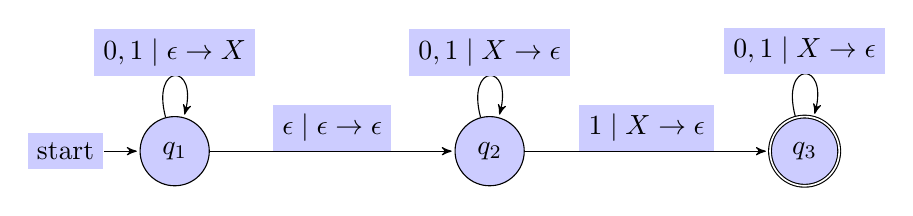
\begin{tikzpicture}[>=stealth',shorten >=1pt,auto,node distance=4cm,every node/.style={fill=blue!20}]
\node[initial,state]   (q1)      				{$q_1$};
\node[state] 	  (q2) [right of=q1]  	{$q_2$};
\node[state,accepting]  	(q3) [right of=q2]  	{$q_3$};


\path[->] (q1)  edge[loop above]	  	node{$0,1 \mid \epsilon \rightarrow X$ } 	(q1)
edge		node{$\epsilon \mid \epsilon \rightarrow \epsilon$}		(q2)
(q2) edge[loop above]  node{$0,1 \mid X \rightarrow \epsilon$} 		 	(q2)
edge node{$1 \mid X\rightarrow \epsilon$}		(q3)
(q3) edge [loop above]  node{$0,1 \mid X \rightarrow \epsilon$}    (q3);
\end{tikzpicture}

\subsection*{b.}

$S\rightarrow X1\\
X\rightarrow X1 \mid X0 \mid 0X \mid 1X \mid \epsilon$
\end{document}




